%%%%%%%%%%%%%%%%%%%%%%%%%%%%%%%%%%%%%%%%%%%%%%%%%%%%%%%%%%%%%%%%%%%
%                                                                 %
%                            CHAPTER SIX                          %
%                                                                 %
%%%%%%%%%%%%%%%%%%%%%%%%%%%%%%%%%%%%%%%%%%%%%%%%%%%%%%%%%%%%%%%%%%%

\chapter{CHANGE DISTANCE} \label{ch:distance}

\section{Introduction}

Use Case 2 addresses the use of versions to communicate how different two objects are.
Many versioning systems use dot-decimal identifiers to signify whether a change is large, medium, or small.
The exact requirements to determine change size differs widely across different domains and applications.
The versioning graph provides a new, more regular method to quantify change between objects using versioning operations.
The work done with GCMD Keywords shows the qualitative relationship between version identifiers and change distance.
Work with the MBVL data set then extends VersOn to give more detailed accounting with the change capture method.

\section{Utilized Data Sets}

\subsection{GCMD Keywords}

The Global Change Master Directory (GCMD) is a metadata repository used by NASA to store records of its available data sets \cite{Miled:2001:GCM:372202.372324}.
They employ a set of keywords to make NASA Earth Science data sets searchable.
These words tag and label datasets into strictly defined categories \cite{GCMDKey}.
GCMD Keywords do not qualify as a standard web ontology since it does not constitute a class hierarchy.
The management team stored early versions of the keywords in Excel spreadsheets, and a centralized distribution system was not used until June 12, 2012.
The Key Management Service now serves the keywords directly in a variety of formats.
Each version of the keywords, encoded in RDF, were downloaded into separate files.
Only versions from June 12, 2012 and after were available, resulting in 9 version files.
Each keyword corresponds to a unique identifier, and when combined with a web namespace, resolves to a data description of the keyword.
Every identifier can be referred to per version by including the version's number at the web identifier's end, meaning that identifiers are consistent across versions.
The taxonomy uses the concepts \textit{skos:Broader} and \textit{skos:Narrower}, where skos refers to the Simple Knowledge Organization System ontology name space, to form a tree hierarchy \cite{skos}.
The tree's root is the keyword, "Science Keywords."
The data set provides an interesting study case due its long sequence of versions and ready use of linked data technology \cite{Stevens2016}.

\subsection{MBVL Classifications} \label{sec:MBVL}

The Marine Biodiversity Virtual Laboratory (MBVL), based at Woods Hole Oceanographic Institution, provides data and services for the study of marine biology with an integrative approach \cite{mbvl}.
In the application studied, a choice of algorithm and taxonomy pairings must be tested on a known population in order to estimate their performance with an unknown microbial population.
The original sequences belong only to the species listed in Table \ref{species_table}.
The original population's census is not available to the author, and only the list of species are known, forming the first data set in this section.
These sequences are then grouped and classified by a specific taxonomy and algorithm pairing.
The workflow utilizes two taxonomies, the Ribosomal Database Project (RDP) and the Silva taxonomy.
Using these databases, the Species-level IdentificatioN of metaGenOmic amplicons (SPINGO) or the Global Alignment for Sequence Taxonomy (GAST) algorithms assign taxonomic ranks to each sequence.
The process produces four data sets, each using the same grouping identifiers and having the same size in each group.
Since the data sets have the same number of sequences, the primary difference between the data sets are the ranks assigned to each sequence.

\begin{table}
	\caption{List of species in the original population.}
	\label{species_table}
	\centering
	\setlength{\tabcolsep}{2pt}
	\begin{tabular}{|c|c|c|}
		\hline
		Acinetobacter baumannii & Actinomyces odontolyticus & Bacillus cereus \\
		Bacteroides vulgatus & Clostridium beijerinckii & Deinococcus radiodurans \\
		Enterococcus faecalis & Escherichia coli & Helicobacter pylori \\
		Lactobacillus gasseri & Listeria monocytogenes & Neisseria meningitidis\\
		Porphyromonas gingivalis & Propionibacterium acnes & Pseudomonas aeruginosa \\
		Rhodobacter sphaeroides & Staphylococcus aureus & Staphylococcus epidermidis\\
		Streptococcus agalactiae & Streptococcus mutans & Streptococcus pneumoniae \\
		\hline
	\end{tabular}
\end{table}

\section{GCMD}

\subsection{GCMD Versioning Graph}

The Global Change Master Directory establishes the context that each \textbf{manifestation} of their keyword list are related versions.
Since the unique identifier for each keyword remains the same across versions, they can be used to align a mapping across versions.
\textbf{Additions} and \textbf{invalidations} are detected by checking an identifier's presence within both versions.
A \textbf{modification} occurs when a keyword's \textit{skos:Broader} property differs between adjacent versions.
A difference indicates that the word has been moved to a different place within the taxonomy since identifiers do not change across versions and a keyword only has one parent concept.
Changes over consecutive versions can be collected into a single graph using the method in Section \ref{sec:multiver} to chain together versioning graphs.
A change log was generated for each pair of consecutive versions in GCMD Keywords and embedded with JSON-LD.
Versioning graphs for each adjacent version was created by extracting JSON-LD from the corresponding change log, and entering the triples into a Fuseki triple store.

\subsection{Connecting Change Counts to Identifiers}

The \textbf{add}, \textbf{invalidate}, and \textbf{modify} counts for each transition are presented in Figure \ref{GCMDC1}.
The query used to extract the counts is found in Listing \ref{gcmd_list}.
Notice the sharp spike in adds and invalidates when transitioning from version 8.4.1 to 8.5.
The version identifiers indicate that at most a minor or technical change has occurred, but the counts of \textbf{addition} and \textbf{invalidation} changes in this transition is more than triple the counts in either of the previous \textbf{major} transitions.
Not only should a small transition not produce changes of this quantity, but the data set's size is on the order magnitude of the recorded \textbf{invalidates}.
In addition, no \textbf{modifications} are revealed, and even the root node "Science Keywords" has been invalidated.
Further investigation of the root word reveals that the name space for the keywords has changed from HTTP to HTTPS.
To provide context, NASA mandated a transition to secure protocols, and the group changed the name space to ensure the URIs remained resolvable.
Since the identifiers are unique, the new name space means they no longer refer to the same object after the protocol change.
Because the keyword identifiers no longer match, the mapping approach results in the total invalidation of keywords from 8.4.1 and the addition of keywords from 8.5.
The dot decimal identifier for the transition from version 8.4.1 to 8.5 does not match the number of changes in the versioning graph.

\begin{table}
	\caption{Global Change Master Directory Keyword Change Counts}
	\label{table:GCMD_main}
	\centering
	\begin{tabular}{|c|c|c|c|c|}
		\hline
		
		Transition&	Add&	Invalidate&	Modify&	Total\\\hline
		June 12, 2012 to 7.0&	310&	9&	22&	341\\
		7.0 to 8.0&	503&	6&	79&	588\\
		8.0 to 8.1&	277&	28&	22&	327\\
		8.1 to 8.2&	53&	1&	26&	80\\
		8.2 to 8.3&	58&	0&	13&	71\\
		8.3 to 8.4&	53&	0&	1&	54\\
		8.4 to 8.4.1&	86&	13&	8&	107\\
		\hline
	\end{tabular}
\end{table}
\begin{figure}[b]
	\centering
	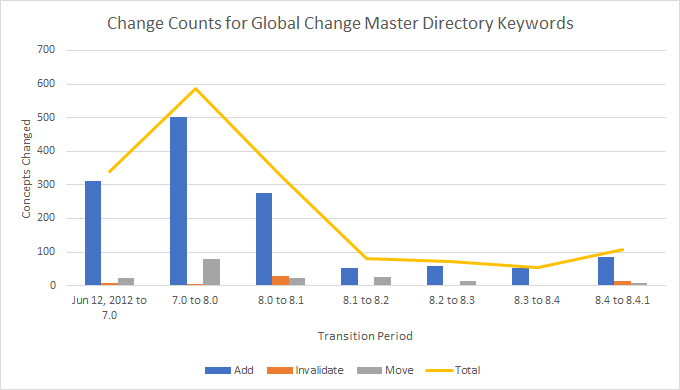
\includegraphics[scale=0.83]{figures/GCMDChartShort.png}
	\caption[Global Change Master Directory Keywords Change counts up to Version 8.4.1]{Add, Invalidate, and Modify counts from the beginning of the Keyword Management System to Version 8.4.1.}
	\label{GCMDC1}
\end{figure}

%\hfill \break
\begin{lstlisting}[language=SPARQL, caption=This query compiles the counts for each subclass of Change in a GCMD versioning graph,label=gcmd_list]
PREFIX vo:<http://orion.tw.rpi.edu/~blee/VersionOntology.owl>
PREFIX rdfs:<http://www.w3.org/2000/01/rdf-schema#>

SELECT ?p (COUNT (DISTINCT ?s) as ?count)
{
?s a ?p .
?p rdfs:subClassOf vo:Change .
} GROUP BY ?p
\end{lstlisting}

Changing the mapping method to account for the new namespace provides a pathway to compare the perceived change by the producer as evidenced by the version identifier with the amount of change in the versioning graph.
To do this, the mapping treats identifiers with HTTP and HTTPS the same. 
Differences in change magnitudes become much clearer after controlling for the altered name space in Figure \ref{GCMDC2}.
All revisions are dominated by \textbf{additions}, but major version changes have counts around 300 to 500 while minor revisions are an order of magnitude smaller.
The transition from version 8.4.1 to 8.5 also seems to follow this trend.
The \textbf{additions} in ``8.4 to 8.4.1" in Figure \ref{GCMDC2} numbers almost a hundred, providing evidence that the trend of decreasing order of magnitudes may now continue as the granularity of the version identifier increases.

\begin{table}
	\caption{Difference in Version 8.5 mapping methods}
	\label{table:GCMD_8_5}
	\centering
	\begin{tabular}{|c|c|c|c|c|}
		\hline
		Mapping Method&	Add&	Invalidate&	Move&	Modify\\ \hline
		Standard&	3097&	3031&	0&	0\\
		Silent&	68&	2&	22&	0\\
		Bridged&	68&	2&	22&	3007\\		
		\hline
	\end{tabular}
\end{table}
\begin{figure}%[b]
	\centering
	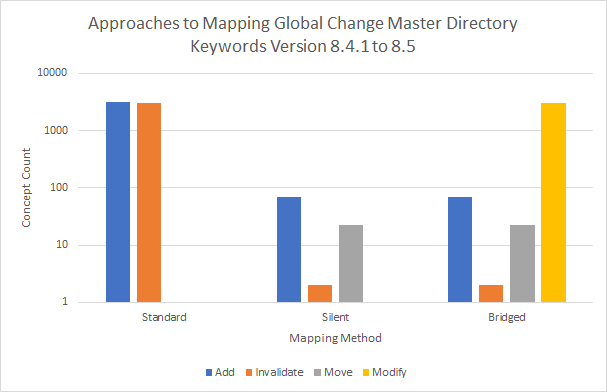
\includegraphics[scale=.9]{figures/GCMD8_5.png}
	\caption{Add, Invalidate, and Modify counts using different methods of mapping identifiers in Global Change Master Directory Keywords Version 8.4.1 to 8.5.}
	\label{GCMDC2}
\end{figure}

\begin{figure}%[b]
	\centering
	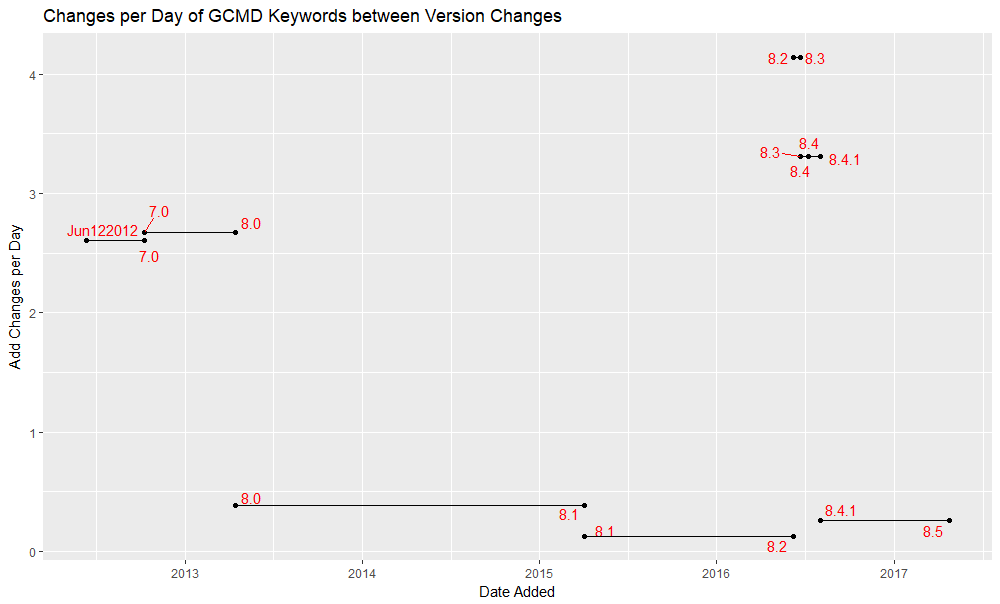
\includegraphics[scale=0.56]{figures/GCMDPlot1.png}
	\caption[Global Change Master Direcotry counts distributed over time.]{Add counts for all versions of GCMD up to 8.5 evenly distributed over the time of version validity.}
	\label{GCMDPlot1}
\end{figure}
\begin{figure}%[b]
	\centering
	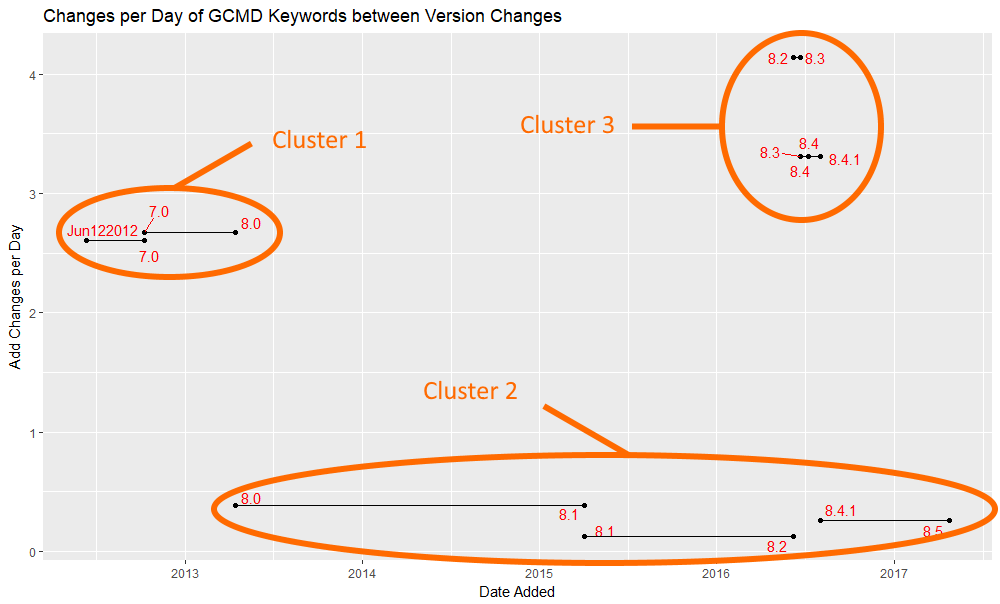
\includegraphics[scale=0.56]{figures/GCMDPlot1_Cluster.png}
	\caption[Global Change Master Directory count distributed over time with clusters marked.]{The change rate of different versions organize into three visible clusters. Cluster 2 denotes a sudden burst of version releases which is notable.}
	\label{GCMDPlot1Cluster}
\end{figure}
\begin{table}
	\caption{Global Change Master Directory versions with old start time changes.}
	\label{table:GCMD_old}
	\centering
	\begin{tabular}{|c|c|c|c|c|}
		\hline
		Version Name&	Publish Date&	2008&	2014&	2015\\ \hline
		8.2&	June 7, 2016&	0&	4&	2\\
		8.3&	June 21, 2016&	0&	7&	1\\
		8.4&	July 7, 2016&	5&	0&	1\\
		\hline
	\end{tabular}
\end{table}

\begin{table}
	\caption{Differences in VersOn and Impact Assessment metrics}
	\label{table:GCMD_metric}
	\centering
	\begin{tabular}{|r|r|r|r|}
		\hline
		Version & Add & Invalidate & Modify\\ \hline
		8.2(VO)&	53&	1&	26\\
		-8.2(IA)&	48&	0&	4\\
		\hline
		&	5&	1&	22\\
		\hline
		8.3(VO)&	58&	0&	13\\
		-8.3(IA)&	58&	0&	10\\
		\hline
		&	0&	0&	3\\
		\hline
		8.4(VO)&	53&	0&	1\\
		-8.4(IA)&	66&	0&	5\\
		\hline
		&	-13&	0&	-4\\
		\hline
		8.5(VO)&	68&	2&	22\\
		-8.5(IA)&	55&	0&	30\\
		\hline
		&	13&	2&	-8\\						
		\hline
	\end{tabular}
\end{table}

\section{MBVL}

\subsection{Variant Versioning Graph}

The experiment conducts activity over two phases in this procedure.
The first phase takes sequences from the original known population and feeds the sequences though a particular algorithm/taxonomy combination to produce a candidate classification.
Since the classifications for the known population sequences is unavailable, there is not sufficient context to perform a valid comparison with the candidate classifications.
The second phase compares the performances of each candidate classification of a algorithm/taxonomy pair.
The use of \textbf{add}, \textbf{invalidate}, and \textbf{modify} varies slightly in this application since all the results use the same sequences.
A versioning graph utilizing just the sequence identifiers would only result in \textbf{modify} changes when taxonomic ranks differ since the sequence identifier exists in both data sets.
The mapping instead uses the sequence identifiers to align comparisons and then the taxonomic rank classification to determine the kind of change.
If the right-hand result specifies more taxonomic ranks, the relationship is an \textbf{addition}.
If the left-hand result is more specific, then the relationship is classified as an \textbf{invalidation}.
If both results have the same precision but the name differs, then the link is a \textbf{modification}.
Otherwise, no change is detected.

Figure \ref{mbvl_chart} shows the changes detected when varying either the taxonomy or the classification algorithm.
\begin{figure}
	\centering
	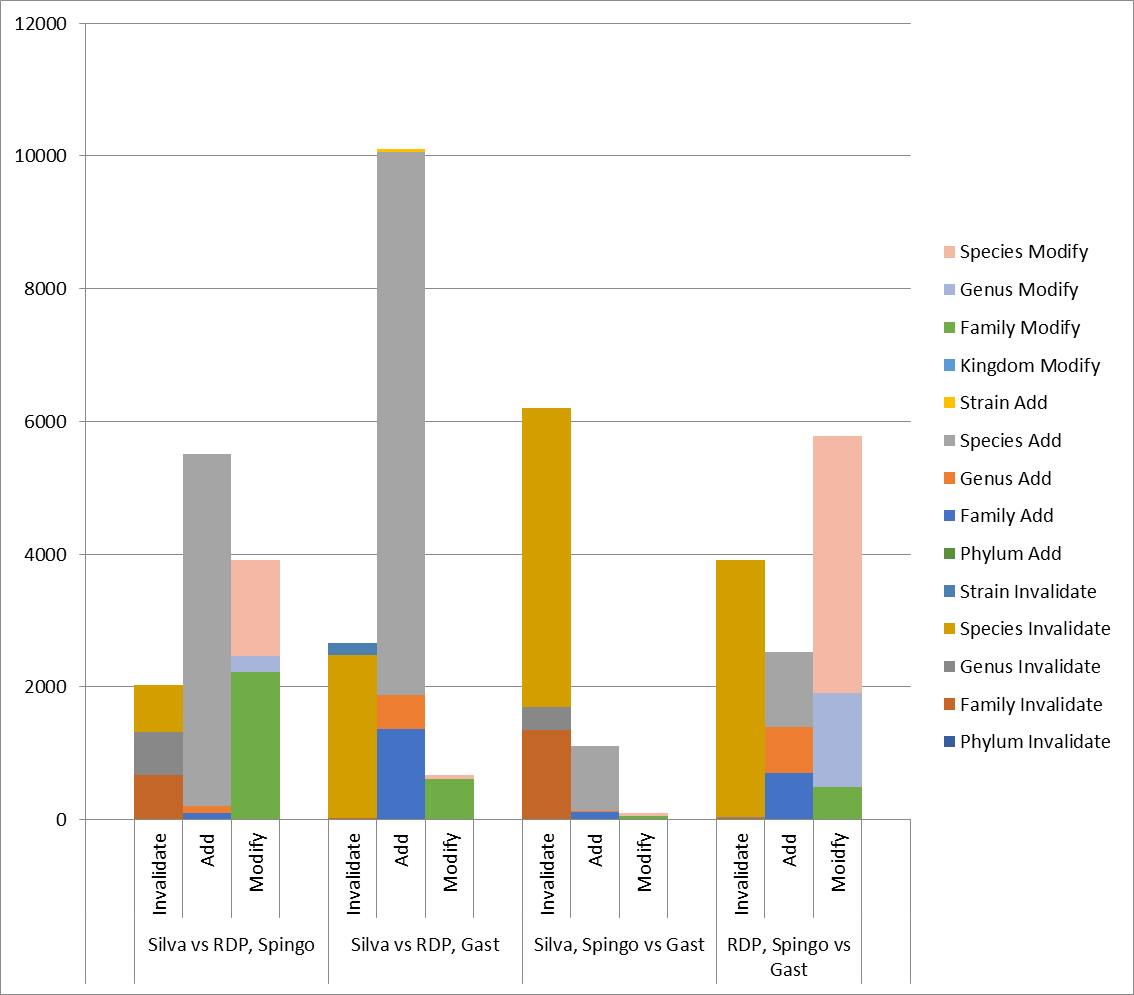
\includegraphics[scale=0.75]{figures/mbvl_chart.png}
	\caption{Compiled counts of \textbf{adds}, \textbf{invalidates}, and \textbf{modifies} grouped by taxonomic rank across algorithm and taxonomy combinations.}
	\label{mbvl_chart}
\end{figure}
No comparison was conducted with different taxonomy and classifier since that would introduce too many sources of variability to differing results in a classification.
Each bar indicates the total number of differences between sequences for a specific kind of change.
The bars are further broken down by the taxonomic rank at which the difference occurred.
For example, in ``Silva vs RDP, Gast", a notable number of classifications differed at the species rank.
The graph also indicates that using the RDP taxonomy often produces more precise classifications since both ``Silva vs RDP, Spingo" and ``Silva vs RDP, Gast" feature a larger number of \textbf{additions} than any other change.
The classifier comparisons feature a high number of \textbf{invalidations}; however, ``RDP, Spingo vs Gast" also displays a higher number of \textbf{modifications} than \textbf{invalidations}.

\section{Analysis}

\subsection{Version Identification}

The versioning process discovered a discrepancy in the identifier assignment in the GCMD Keywords taxonomy.
The original analysis was intended to determine if dot-decimal identifiers could be predicted using the change counts of the versioning graph.
Version 8.5, however, was named with respect to perceived taxonomy changes and did not consider underlying linked data practice revisions.
The disconnect brings into question the accuracy of all prior names and any relationships observed between identifier and change counts.
Non-matching identifiers would explain how 8.4.1 had more additions than any previous minor change but obtains a third bracket identifier.
After accounting for namespace differences in version 8.5, the change counts is in the tens, resembling tallies of other versions in the same identifier bracket.
Version name assignment based on producer perception and not on more concrete measures is concerning.
An incomplete understanding in the amount of change between two versions can lead to flawed expectations during version migration.

The analysis does not to claim that change counts should be the sole mechanism in determining version identifiers.
The counts, however, can provide a more quantitative method to compare version differences.
In Figure \ref{GCMDC2}, the yellow line indicates the total changes made to the data set, performing a similar function as the major/minor/revision version identifier.
Breaking up the changes into types reveals additions dominate manipulations to the data set.
Addition, invalidation, and modification provides deeper insight into how a data set is changing, but some changes can be more impactful than others which this model does not capture.

\subsection{MBVL Analysis}

In Chapter \ref{ch:distance}, the versioning process was used to compare the performance of different taxonomy and algorithm combinations.
The data set diverges from many of the common understandings of versions since each of the versions are not sequential and are largely independent.
The data set of species names in the initial population would not have produced very meaningful results if applied to the versioning model since it lacked sufficient data to map the other data sets together well.

In Figure \ref{mbvl_chart}, the first set of columns in the Silva taxonomy results are versioned against RDP using the SPINGO algorithm.
The naming reflects the orientation in the versioning graph so Silva forms the left-hand version and RDP would be the right-hand version.
In this comparison, using the RDP taxonomy seems to provide more accurate results, most specifically at the species level.
The taxonomies also disagree fairly often at the species and family ranks.
Switching to the GAST algorithm in the second set of columns, RDP once again demonstrates a noticeably greater accuracy in species classification.
There are also significantly fewer disagreements using the GAST algorithm between the two taxonomies.
Looking at the third set of columns, Silva demonstrates greater accuracy classifications under the SPINGO algorithm than under GAST.
Over four thousand of these entries can be classified to the species level when GAST cannot.
In the fourth set of columns, RDP appears to perform better with SPINGO than GAST.
However, the comparison is dominated by a much larger number of disagreements between almost six thousand entries, primarily at the species rank.
On closer inspection, this disagreement is explained by GAST classifying the species for a number of entries as ``uncultured bacterium".
This analysis presents evidence that using the RDP taxonomy with the SPINGO algorithm will produce the most accurate classification results.

\section{Summary}

The result of testing the second hypothesis is inconclusive.
Initial results suggested that identifier assignment and version change size followed an order scale, major changes numbered in the hundreds while minor changes were associated with tens of adds.
The behavior of version 8.5, however, brings into question how accurate or subjective any of the identifiers may be.
Verifying the accuracy of the change counts becomes invalid without further study using other works.
The version graph method does provide a more nuanced view of the distance measure by dividing the total number of changes into groups by operation.
The observation that invalidations almost equaled addition in an add dominated data set in the 8.4.1 to 8.5 transition provided evidence that the data set was completely deleted and an entirely new one added.

The MBVL data set demonstrates a case where versioning graphs can be used to compare the performance of different taxonomy/algorithm pairings.
The ability derives from sub-classing each of the add, invalidate, and modify changes to give a better perspective where the pairings differed.
This approach of extending the versioning graph adds domain knowledge to the version comparison and helps contextualize the observed differences.